%%%%%%%%%%%%%%%%%%%%%%%%%%%%%%%%%%%%%%%%%%%%%%%%%%%%%%%%%%%%%%%%%%%%%%%%%%%%%%%%
%2345678901234567890123456789012345678901234567890123456789012345678901234567890
%        1         2         3         4         5         6         7         8

\documentclass[letterpaper, 10 pt, conference]{ieeeconf}  % Comment this line out
                                                          % if you need a4paper
%\documentclass[a4paper, 10pt, conference]{ieeeconf}      % Use this line for a4
                                                          % paper

\IEEEoverridecommandlockouts                              % This command is only
                                                          % needed if you want to
                                                          % use the \thanks command
\overrideIEEEmargins
% See the \addtolength command later6 in the file to balance the column lengths
% on the last page of the document



% The following packages can be found on http:\\www.ctan.org
\usepackage{graphics} % for pdf, bitmapped graphics files
%\usepackage{epsfig} % for postscript graphics files
%\usepackage{mathptmx} % assumes new font selection scheme installed
%\usepackage{times} % assumes new font selection scheme installed
\usepackage{amsmath} % assumes amsmath package installed
%\usepackage{amssymb}  % assumes amsmath package installed
\usepackage{graphicx}
% \usepackage{subfig}
\usepackage{subcaption}
\usepackage{booktabs}
\usepackage{float}
\title{\LARGE \bf
A Less-Dependent Threshold Corner Detection Algorithm
}

%\author{ \parbox{3 in}{\centering Huibert Kwakernaak*
%         \thanks{*Use the $\backslash$thanks command to put information here}\\
%         Faculty of Electrical Engineering, Mathematics and Computer Science\\
%         University of Twente\\
%         7500 AE Enschede, The Netherlands\\
%         {\tt\small h.kwakernaak@autsubmit.com}}
%         \hspace*{ 0.5 in}
%         \parbox{3 in}{ \centering Pradeep Misra**
%         \thanks{**The footnote marks may be inserted manually}\\
%        Department of Electrical Engineering \\
%         Wright State University\\
%         Dayton, OH 45435, USA\\
%         {\tt\small pmisra@cs.wright.edu}}
%}

\author{Yihui Li, Yan Huang, Yijiong Lin, Haifei Zhu and Yisheng Guan$^{*}$   % <-this % stops a space
%\thanks{*This work was not supported by any organization}% <-this % stops a space
\thanks{ 
All authors are with the Biomimetic and Intelligent Robotics Lab (BIRL), the School of Electro-mechanical Engineering, Guangdong University of Technology, Guangzhou, China. Y. Guan is the corresponding author, email: {\tt\small ysguan@gdut.edu.cn}.}
\thanks{
The work in this paper is supported in part by the NSFC-Guangdong Joint Fund (Grant No. U1401240), the Natural Science Foundation of Guangdong (Grant No. 2015A030308011), and the Frontier and Key Technology Innovation Special Funds of Guangdong (Grant Nos. 2015B010917003, 2017B050506008).}
}
\begin{document}



\maketitle
\thispagestyle{empty}
\pagestyle{empty}


%%%%%%%%%%%%%%%%%%%%%%%%%%%%%%%%%%%%%%%%%%%%%%%%%%%%%%%%%%%%%%%%%%%%%%%%%%%%%%%%
\begin{abstract}

Existing corner detection algorithms excessively depend on the selection of thresholds, which result in complex implementation and unstable performance. Our purpose is to weaken the influence of threshold in corner detection. This paper presents a less-dependent threshold corner detection method to extract geometrically important corners for image vectorization. In general, the performance of the existing corner detection algorithm depends largely on one or more thresholds. Specifically, corner candidates are extracted with an improved intensity-based detector and contour-based detector, respectively. The corner candidates are classified into two groups: uncertain corners and certain corners which are sorted by a matching method based on Euclidean distance. With the certain corners, we define Self-confident Level (SCL), which does not depend on any threshold, to remove false corners from the uncertain corners. Experiments validate the good performance of the proposed method.

\end{abstract}
%%%%%%%%%%%%%%%%%%%%%%%%%%%%%%%%%%%%%%%%%%%%%%%%%%%%%%%%%%%%%%%%%%%%%%%%%%%%%%%%
\section{INTRODUCTION}
Corners provide significant information to describe object features and hence play an important role in various applications, such as object recognition, motion tracking, image registration, stereo matching and so on. Our interest in the problem of corner detection is derived from the desire of ornamental image vectorization in ceramic tiling automation. Contours of the ornamental images need to be vectorized and finally converted to CAD files, which can be used in water-jet cutting and robot tiling. In the process, corners can be tracked as features to extract and parameterize the contours. 

Much work has been done on corner detection in the past decades. Generally, these methods can be classified into three categories \cite{Kahaki2014Contour}: intensity-based detector, contour-based detector, and model-based detector. They are applied to different conditions and fields with different features. 

Model-based detectors extract corners by matching image patches with the predefined models. Krishnan proposed an optimal corner detector using a mathematical model for a corner \cite{Brackle1989Optimal}. Gustavo and Benjamin introduced a parametric corner model which can be used to model and identify a certain class of characteristic intensity variation based on a Unit Step Edge Function \cite{Olague2005}. Sinzinger presented an approach to junction detection using radial energy \cite{Sinzinger2008A}. This approach fits the neighborhood around a point to a junction model which segments the neighborhoods into wedges by determining a set of radial edges. The radial edges are invariant to affine transforms and creating an affine invariant junction detector. Florentz and Aldea used a corner occurrence model to predict the optimal threshold for a predefined number of detections \cite{Florentz2014SuperFAST}, this method is efficient in term of time since it avoids scoring and sorting the detected corners. Generally, the predefined models which are equivalent to thresholds cannot cover all corners in real images, limiting their performance in various application \cite{Shui2013}. 

Contour-based detectors generally consist of three cascaded steps: edge detection, contour extraction, and corner decision on contours \cite{Shui2013}. The most popular and widely used ones are based on curvature scale space (CSS) due to their high performance \cite{Kitchen1982Gray}\cite{Kim2012Robust}. Various methods are proposed based on Mokhtarian's idea which introduced the basic CSS-based method \cite{Mokhtarian1992A}. He and Yung proposed an improved multi-scale corner detector with adaptive threshold instead of a single global threshold as in the original CSS method, and false corners are eliminated by a dynamic region of support \cite{He2004Curvature}. In Zhang's method, local extremums of the curvature product exceed the predefined threshold at different scales are identified as corners \cite{Zhang2007Multi}. Topal proposed a robust CSS detector based on the turning angle curvature of image gradients \cite{Topal2013A}. CSS-based detectors are sensitive to noise on the contour and time-consuming because of using high derivatives to compute curvature, and whose performance depends largely on the quality of edge detection, in other words, the thresholds make an important role.

Intensity-based detectors extract corner by comparing the local grayscale variation of image \cite{Kahaki2014Contour}. Kitchen and Rosenfeld proposed a corner detection scheme based on a differential operator which determines the first and second partial derivatives of image, and the local extrema one is identified as corner \cite{Kitchen1982Gray}. This method is noise-sensitive so that the detection and localization accuracy is poor. Based on Moravec's method \cite{Morevec1977Towards}, Harris and Stephen proposed a detector using approximates of the gradient auto-correlation in each direction \cite{Harris1988A}. This method has good performance in rotation and various illuminations, but suffers from a loss in localization accuracy and is only robust in L-type corners \cite{Noble1988Finding}. Tomasi improved Harris' detector by a small correction and calculating the minimum eigenvalues \cite{Shi1993Good}. Smith and Brady proposed the SUSAN detector using a circular mask for corner and edge detection \cite{Smith1997SUSAN}. Although the localization and noise robustness of SUSAN detector are better than the aforementioned detector, it is time-consuming when calculating the USAN area and finding the corners in the whole image window. More importantly, it's difficult to confirm the threshold by which to distinguish corners from edge. Although intensity-based detectors are more popular in application, gray-scale methods are not so accurate to locate the exact corners \cite{Kahaki2014Contour}. Some novel techniques, such as deep learning, are applied in corner detection recently \cite{lei2004cnn}\cite{Dong2018Corner}.

In summary, intensity-based corner detectors have good anti-noise performance, but the corner localization accuracy and performance of detecting obtuse angles are not satisfied. Moreover, their performance depends to large extent on the threshold of intensity. On the other hand, contour-based corner detectors can detect structural corners, but they are sensitive to noise on the contour and their performance depends severely on the performance of edge detection and the angle threshold. Therefore, it is necessary to eliminate or weaken the influence of threshold in corner detection, which is the motivation of the method presented in this paper. 

This paper is organized as follows. Section II introduces the overall framework and the detailed idea of the proposed method. Experiments, performance comparison are presented and discussed in Section III. Finally, we make a conclusion in Section IV.

\section{Proposed Method}

\subsection{Overview}

As mentioned before, the performance of the existing corner detection methods depends largely on the threshold, and therefore an algorithm to eliminate or weaken the influence of threshold in corner detection is desired. The algorithm presented in this paper achieves this goal. In our algorithm, corner candidates are extracted with an improved intensity-based detector and contour-based detector, respectively. Then based on Euclidean distance, the same corners between two corner sets are matched. With the matched corners, we define Self Confident Level (SCL), which does not depend on any threshold, to remove false corners from the unmatched corners. The method can be described as follows.

1. With the basic idea of Harris detector \cite{Harris1988A} and CSS detector \cite{He2008Corner}\cite{Mokhtarian}, corners are extracted with a low threshold so that as many as corners can be included in the set of corner candidates (false corners may be included too). 

2. The matched points located between the two corners sets based on Euclidean distance. 

3. The Self Confident Level (SCL) is computed based on corner response score \cite{Harris1988A} and corner angle for each unmatched corner, respectively. The SCL is used to eliminate false corners from the corner candidates in leak detection procedure.

\subsection{Corner Candidates}
Different from general detectors which use a single method to obtain corner candidates, our method applies Harris and an improved CSS detector to extract two independent corner sets which make up the corner candidates. To weaken the threshold dependency of these two detectors, an improvement is made in this procedure. To begin with, we discuss threshold influence of the two detectors and the improvement below.

Harris detector \cite{Harris1988A} is an intensity-based corner detection method. It takes the differential of the corner score into account with reference to direction directly, instead of using shifting patches for every 45 degrees angle, and has been proved to be more accurate in distinguishing between edges and corners \cite{Dey2012A}. A corner response score ${R}$ is defined in this detector as follows:
\begin{equation}
\begin{split}
R = \operatorname { det } ( M ) - k*( \operatorname { trace } ( M ) ) ^ { 2 }
\end{split}
\label{corner response score}
\end{equation}
where ${M}$ is the structure tensor of the processing image, ${M=\lambda _ { 1 }+\lambda _ { 2 }}$, ${\lambda _ {1}}$ and ${\lambda _ {2}}$ are eigenvalues of ${M}$. ${det(M)}$ is the determinant of ${M}$, ${trace(M)}$ is the trace of ${M}$ and ${k}$ is an empirically determined constant, ${k \in [ 0.04,0.06 ]}$. Figure \ref{corner response score property} shows the property of ${R}$ indicating that:

1. ${R}$ depends only on the eigenvalues of ${M}$.

2. ${R}$ is large for a corner region.

3. ${R}$ is negative with large magnitude for an edge region.

4. ${|R|}$ is small for a flat region.

A threshold of ${R}$ is used to determine whether a corner candidate is true corner or not in the original Harris method, that is, if ${R(i) > R _ { threshold }}$, then the ${i-th}$ corner is considered as a true corner. However, it's difficult to determine exact ${R _ { t }}$ which plays a decisive role of the number of true corners. In order to ensure as many as true corners are included in corner candidates, ${R _ { t }}$ is given by:
\begin{equation}
\begin{split}
{R _ { t }} = t * R _ { \operatorname { max } }
\end{split}
\label{corner response score threshold}
\end{equation}
where ${R _ { max }}$ is the maximum of ${R}$, ${t}$ is a coefficient of ${R _ { max }}$, which is a small value so that as many as corners can be included in the corner candidates, and can be matched in later procedure. A value ${t = 0.0001}$ has been used in all experiments presented in this paper.
\begin{figure}[htbp]
\centering
%\includegraphics[width=8cm]{corner_response_score.png}
\includegraphics[width=.9\linewidth]{experiments/corner_response_score.png}
\caption{The property of corner response score ${R}$.}
\label{corner response score property}
\end{figure}

CSS detector is a contour-based corner detection method. Based on the curvature scale space technique, corners are detected at a high scale of the CSS and the locations are tracked through multiple lower scales to improve localization. Different from the original CSS detector using multiple curvature scales to extract corners, we quote an enhanced CSS detector \cite{He2008Corner} which compute a curvature value at a high scale and then consider corners to be defined by global and local curvature properties, to obtain another part of corner candidates. There are two main thresholds involved in the enhanced method: a) grayscale threshold used to detect edges with the Canny detector, b) angle threshold designating the maximum obtuse angle that a corner can have and still be considered as a true corner. For the first one, we adopt OTSU's method \cite{Ohtsu1979A} to ensure an adaptive threshold to obtain the edge map. For another, the parameter ${\theta _ {obtuse}}$ designates the maximum obtuse angle, if the angle of a corner is not larger than ${\theta _ {obtuse}}$, then the corner can be considered as a true corner. A value ${\theta _ {obtuse} = 175}$, close to straight angle has been used in all experiments presented in this paper, so that as many as corners can be included in the corner candidates. 

The final set of corner candidates ${C_{C}}$ can be define as follows: 
\begin{equation}
\begin{split}
C _ { C } = C _ { H } \cup C _ { E }
\end{split}
\label{corner candidates}
\end{equation}
where ${C_{H}}$ is the set of corners detected by Harris detector and ${C_{E}}$ is one detected by the enhanced CSS detector. 

\subsection{Corner Matching}
Generally, a well-defined corner should be detected by detectors based on different principles, this is the reason why we choose two corner detectors in different principles (intensity-based and contour-based) to obtain the corner candidates, which is more persuasive than using two methods in the same principle. Then we consider that the same corners between the two initial corner sets obtained in subsection B. As shown in Fig. \ref{Corner candidates group}, corner candidates are classified into two groups: certain corners and uncertain corners. The certain corners are sorted by Euclidean distance. Since the certain corners are detected by both Harris method and the enhanced CSS method, they are robust in different principles, and hence they are considered as true corners. In detail, if the following condition is met, a corner can be included in the set of certain corners:
\begin{equation}
\begin{split}
\operatorname { max } \sum _ { i = 1 } ^ { M } \sum _ { j = 1 } ^ { N } \| P _ { i } - P _ { j } ^ { \prime } \| \leq d
\end{split}
\label{corner matching_Euclidean distance}
\end{equation}
where ${P _ { i }}$ is the ${i-th}$ corner in ${C_{H}}$ and ${M}$ is the corner numbers of ${C_{H}}$. ${P _ { j } ^ { \prime }}$ is the ${j-th}$ corner in ${C_{E}}$ and ${N}$ is the numbers. ${d}$ is the matching threshold, a value ${d = 3}$ has been used in this paper. Note that ${d}$ is different from the thresholds mentioned above because a certain corner should be robust in different principles. 
\begin{figure}[htbp]
\centering
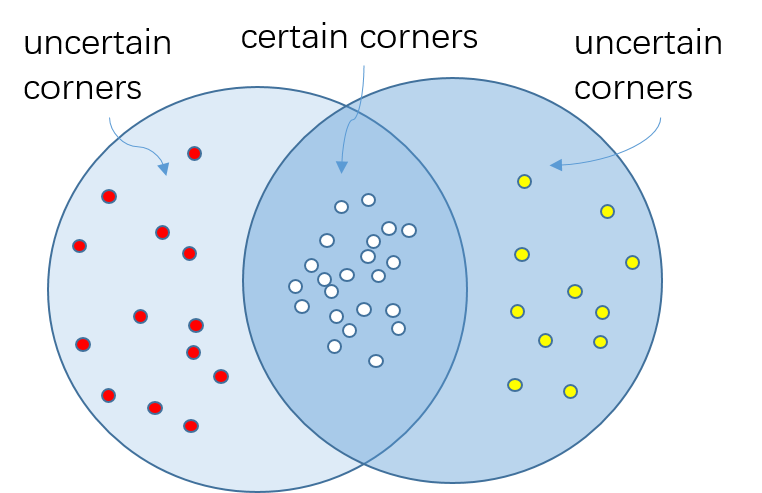
\includegraphics[width=.9\linewidth]{experiments/cetain_uncertain_corners.png}
\caption{Corner candidates group: certain corners and uncertain corners.}
\label{Corner candidates group}
\end{figure}

\subsection{False Corners Removal}

Certain corners are considered as true corners since their robustness. A method is needed to determine whether an uncertain corner should be considered as a false one and removed. Different from the original method using uncertain thresholds of several parameters, we defined Self-confident Level (SCL) to remove false corners from the uncertain corners. SCL does not depend on any threshold, uncertain corners are classified into two parts: the ones detected with the Harris method and those detected with the enhanced method.

For the first part, since corner response score mentioned in Section II is an important parameter to determine whether a point is corner or not, so the SCL of this part is defined as follows:
\begin{equation}
\begin{split}
SCL _ { H } ^ { m } = \frac { R _ { u1 } ^ { m } } { min R _ { c }  }
\end{split}
\label{SCL for Harris}
\end{equation}
for the $m-th$ corner in the first part, ${SCL _ { H } ^ { m }}$ is the SCL, ${R _ { u1 } ^ { m }}$ is the corner response score, and ${ min R _ { c }}$ is the minimum corner response score of all certain corners. If ${SCL _ { H } ^ { m }}$ meets the following condition:
\begin{equation}
\begin{split}
SCL _ { H } ^ { m } \geq 100\%
\end{split}
\label{SCL condition for Harris}
\end{equation}
which means that the corner response score of the $m-th$ corner in the first part is larger than the minimum corner response score of all certain corners, then the $m-th$ uncertain corner can be considered as a true corner. 

For the second part, each corner except for the endpoints in this part has an corresponding angle \cite{He2008Corner}. With this parameter, the SCL of the $n-th$ corner in this part is defined as follows:
\begin{equation}
\begin{split}
SCL _ { C } ^ { n } = \frac { \theta _ { u2 } ^ { n } } { max \theta _ { c }  }
\end{split}
\label{SCL for CSS}
\end{equation}
where $ { \theta _ { u2 } ^ { n } }$ is the angle of $n-th$ corner in the second part, and ${ max \theta _ { c }  }$ is the maximum angle of all certain corners except for the endpoints. If $SCL _ { C } ^ { n }$ meets:
\begin{equation}
\begin{split}
SCL _ { C } ^ { n } \leq 100\%
\end{split}
\label{SCL condition for Harris}
\end{equation}
which means that the angle of the $m-th$ corner in the second part is smaller than the maximum angle of all certain corners, then the $n-th$ uncertain corner can be considered as true corner. 

The loose thresholds (the small corner response score threshold ${R _ { t }}$ and the angle threshold ${\theta _ {obtuse} }$ which is set as nearly close to $180 ^ { \circ }$ in this paper) which used to obtain the corner candidates in Section II results in many false corners escaping. The method to calculate SCLs is actually to search adaptive thresholds for the false corner classification. Moreover, the two adaptive thresholds could be a feedback to iterate and obtain new and more accurate corner candidates, which is not addressed in this paper.

\section{Experiments}
To verify the effectiveness of the presented corner detection method, experiments are conducted in this section. Its performance is also evaluated by comparing with popular corner detection algorithms including Harris detector \cite{Harris1988A}, the enhanced CSS \cite{He2008Corner} and RCSS \cite{Topal2013A}. Note that all parameters of these three detectors are the default values. To evaluate the performance of the proposed method, some published images, planar shapes and images that going to be vectorized are chosen as experimental data.

\subsection{Corner Matching Result}
As shown in Fig. \ref{Corner matching show}, the original images are two same real images of blocks stitched together. Corners on the left are extracted with Harris detector and the ones on the right are extracted with the enhanced CSS method. Almost all true corners are included in the corner candidates because of the preset loose thresholds. However, the number of false corners increase accordingly. Matched corners are lined with green lines. Moreover, almost all matched corners are true. This result verifies that the proposed matching method is effective. 
\begin{figure}[htbp]
\centering
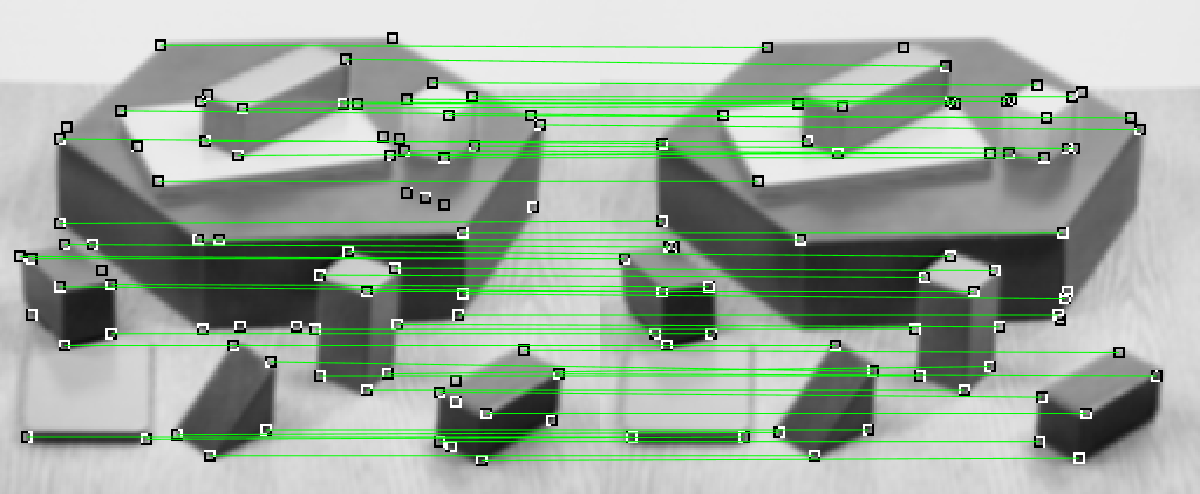
\includegraphics[width=\linewidth]{experiments/blocks_corner_matching.png}
\caption{Corner candidates matching of the "Blocks" images.} 
\label{Corner matching show}
% \centering
% 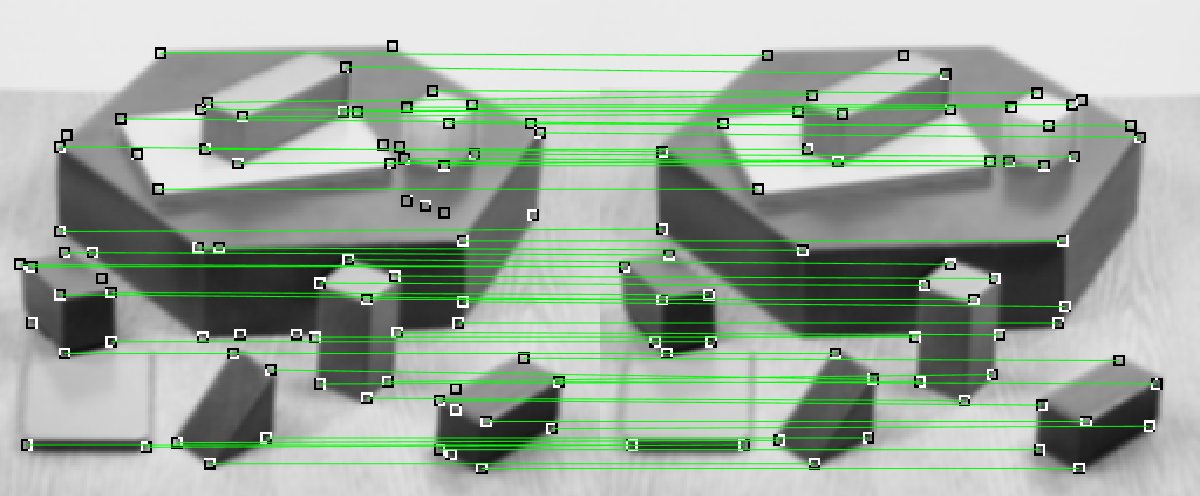
\includegraphics[width=.75\linewidth]{blocks_corner_matching.png}
% \caption{Corner candidates matching of the "Blocks" image} 
% \label{Corner matching show}
\end{figure}

\subsection{Comparison with Ground Truth}
As the most popular test image in corner detection verification, the ”Blocks” image is employed for comparison in this subsection. Since it is difficult to determine whether a point is a corner or not. To perform an objective evaluation, a reference for comparison is needed. Fig. \ref{Results on Blocks image}(a) is the reference solution that we manually generated with the "Blocks" image. The method of evaluation adopted in this research is described as follows \cite{He2008Corner}:  
\begin{figure}[htbp]
	  	\centering
	% \begin{subfigure}[b]{\linewidth}
 %    	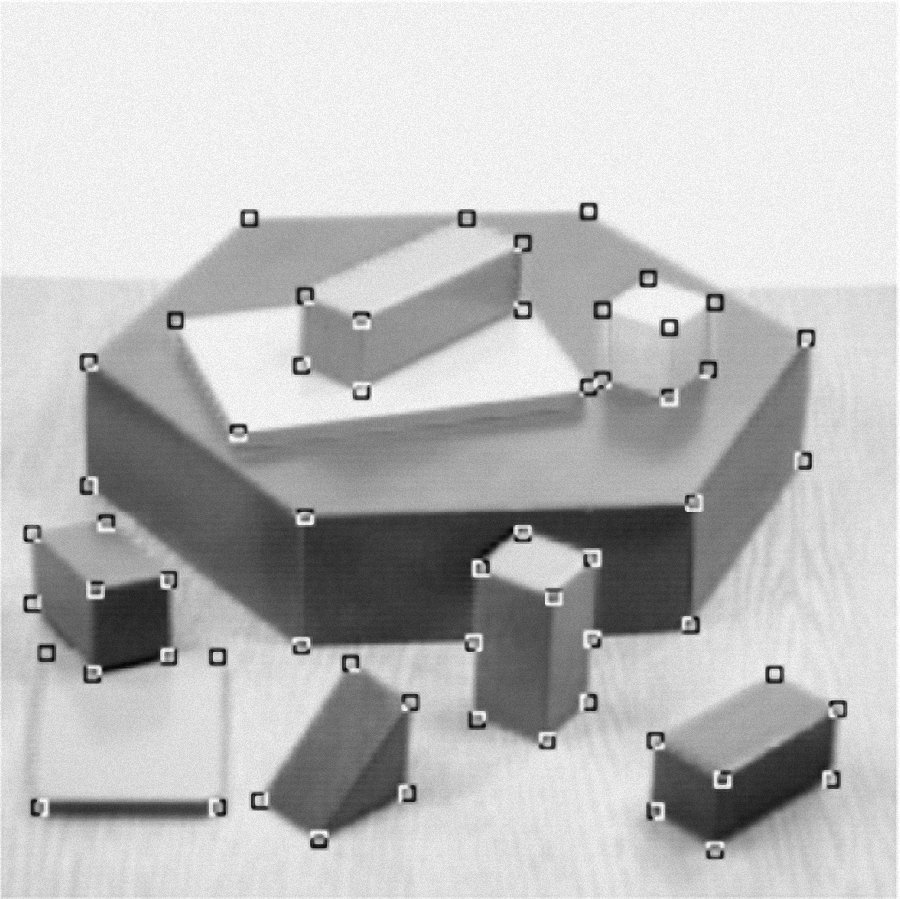
\includegraphics[width=\linewidth]{experiments/blocks_true_corners.png}
 %    	\caption{}
 %   	\end{subfigure}
   	\begin{subfigure}[b]{0.49\linewidth}
    	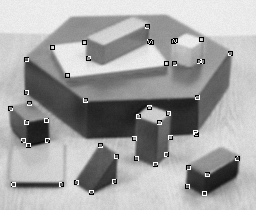
\includegraphics[width=\linewidth]{experiments/blocks_harris.png}
    	\caption{}
   	\end{subfigure}
  	     \begin{subfigure}[b]{0.49\linewidth}
      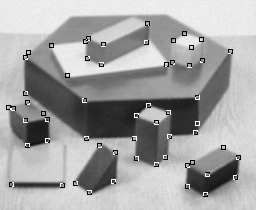
\includegraphics[width=\linewidth]{experiments/blocks_ECSS.png}
      \caption{}
    \end{subfigure}
       	\begin{subfigure}[b]{0.49\linewidth}
    	\includegraphics[width=\linewidth]{experiments/blocks_rcss.png}
    	\caption{}
   	\end{subfigure}
  	     \begin{subfigure}[b]{0.49\linewidth}
      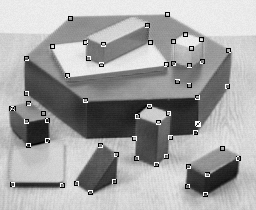
\includegraphics[width=\linewidth]{experiments/blocks_final.png}
      \caption{}
    \end{subfigure}

      	\caption{Detection results on the "Blocks" image: (a) reference solution, (b) Harris, (c) the enhanced CSS, (d) RCSS, (e) proposed method.}
      	      	% \caption{Detection results on the "Blocks" image: (a) Harris, (b) the enhanced CSS, (c) RCSS, (d) proposed method}
  	\label{Results on Blocks image}
	\end{figure}
% \begin{figure*}[htbp]
% 	  	\centering
% 	   	\begin{subfigure}[b]{0.195\linewidth}
%     	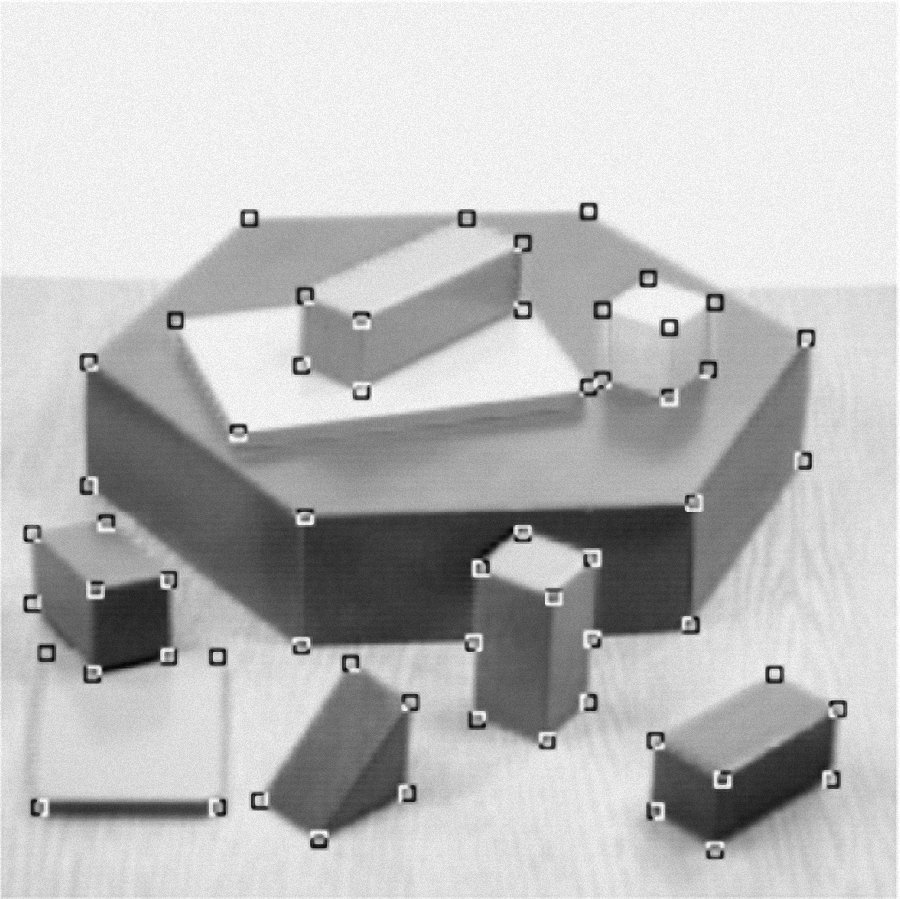
\includegraphics[width=\linewidth]{experiments/blocks_true_corners.png}
%     	\caption{}
%    	\end{subfigure}
%    	\begin{subfigure}[b]{0.195\linewidth}
%     	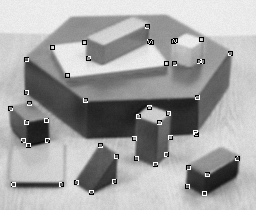
\includegraphics[width=\linewidth]{experiments/blocks_harris.png}
%     	\caption{}
%    	\end{subfigure}
%   	     \begin{subfigure}[b]{0.195\linewidth}
%       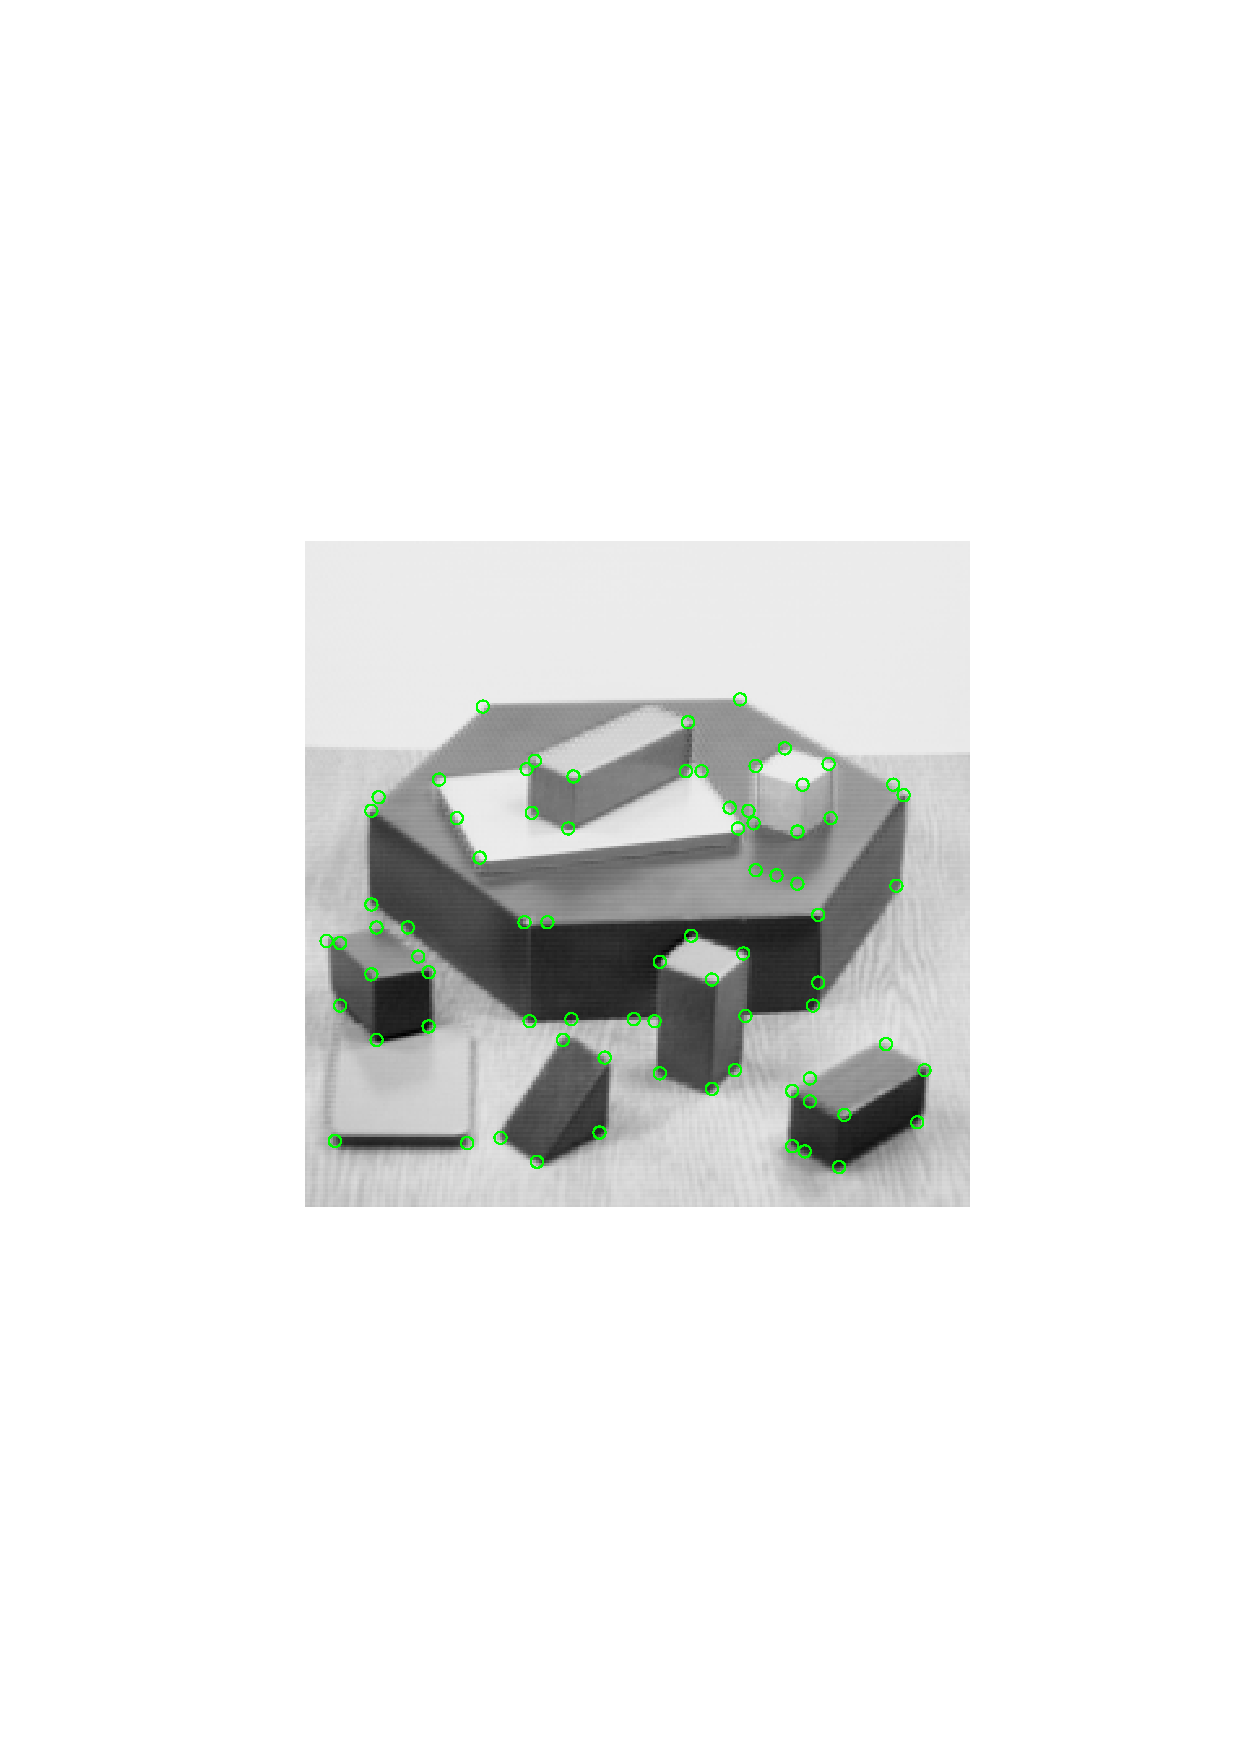
\includegraphics[width=\linewidth]{experiments/blocks_CSS.png}
%       \caption{}
%     \end{subfigure}
%        	\begin{subfigure}[b]{0.195\linewidth}
%     	\includegraphics[width=\linewidth]{experiments/blocks_rcss.png}
%     	\caption{}
%    	\end{subfigure}
%   	     \begin{subfigure}[b]{0.195\linewidth}
%       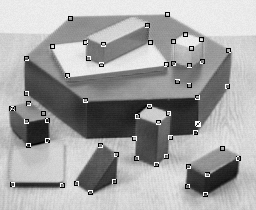
\includegraphics[width=\linewidth]{experiments/blocks_final.png}
%       \caption{}
%     \end{subfigure}
%       	\caption{Detection results on the "Blocks" image: (a)reference solution, (b) Harris, (c) the enhanced CSS, (d) RCSS, (e) proposed method}
%   	\label{Results on Blocks image}
% 	\end{figure*}
\begin{equation}
\begin{split}
d _ { ij} = || C _ { REF } ^ { i } - C _ { COM } ^ { j } ||
\end{split}
\label{evaluation equation}
\end{equation}
where $C _ { REF } ^ { i }$ denotes $i-th$ corner in the corner set of the reference solution, $C _ { COM } ^ { j }$ is $j-th$ corner in the comparison corner set and $d _ { ij}$ is the distance between $C _ { REF } ^ { i }$ and $C _ { COM } ^ { j }$. If $d _ {ij}$ is the minimum for ${i,j}$, and if $d _ {ij} \leq D _ {max} $, then $C _ { COM } ^ { j }$ is labeled as a true corner; otherwise, $C _ { REF } ^ { i }$ is marked as a missed corner. Here $D _ {max}$ is defined to be the maximum admissible distance between $C _ { REF } ^ { i }$ and $C _ { COM } ^ { j }$, which is set to 4 pixels in the following evaluation. The remaining corners in $C _ { COM }$ are considered as false corners. We also assess the efficiency of employed detectors with an evaluation metrics, accuracy (ACU) \cite{Topal2013A}. ACU is defined as follows:
\begin{equation}
\begin{split}
ACU = (N _ { TRUE }/N _ { COM } + N _ { TRUE }/N _ { REF })/2
\end{split}
\label{ACU}
\end{equation}
where $N _ { TRUE }$ is the number of the true corners, $N _ { REF }$ and $N _ { COM }$ are the number of $C _ { REF }$ and $C _ { COM }$, respectively. The comparison with those three other corner detectors are summarized in Fig. \ref{Results on Blocks image} and TABLE \ref{evaluation table}. Fig. \ref{Results on Blocks image}(a) depicts the corners of reference solution and the number of true corners is 59 in the "Blocks" reference solution. The proposed method shows the best performance in this extraction, not only with the number of true corners, missed corners and false corners, but also the ACU is the best as well compared with other detectors. Although choosing with loose thresholds results in many false corners mixing in corner candidates, most of the false corners are removed after leak detection procedure. The two CSS methods perform quite well too and the enhanced CSS method better than RCSS in each items. Due to the difficulty of getting corner response score threshold, Harris detector shows worst performance although its ACU is up to 0.803. In summary, the results highlight the function of weakening the influence of threshold with the proposed method.
%The localization error is calculated as the mean of all the distances $d _ { ij}$ for those correctly detected corners.
\begin{table}[h]
\renewcommand\arraystretch{1.5}
\caption{Evaluation results for the “Blocks” image}
\label{evaluation table}
\begin{center}
\setlength{\tabcolsep}{4mm}{
\begin{tabular}{@{}lcccc@{}}
\toprule
Detector          & \begin{tabular}[c]{@{}c@{}}True\\ corners\end{tabular} & \begin{tabular}[c]{@{}c@{}}Missed\\ corners\end{tabular} & \begin{tabular}[c]{@{}c@{}}False\\ corners\end{tabular} & ACU            \\ \midrule
Harris            & 43                                                     & 16                                                       & 16                                                      & 0.803          \\
Enhanced CSS      & 51                                                     & 8                                                        & 6                                                       & 0.872          \\
RCSS              & 49                                                     & 10                                                       & 10                                                      & 0.831          \\
\textbf{Proposed Method} & \textbf{53}                                            & \textbf{6}                                               & \textbf{6}                                              & \textbf{0.898} \\ \bottomrule
\end{tabular}}
\end{center}
\end{table}

\subsection{Results on Ornamental Images}
The Ornamental images are the origin of water-jet cutting and ceramic tiling automation. Contours of the ornamental images need to be vectorized and finally converted to CAD files, which can be used in water-jet cutting, robot tiling, and any other 2D cutting. In the process, corners can be tracked as features to extract and parameterize the contours. 

In this subsection, two typical ornamental images are used to extract corners with the same detectors as in the last subsection. From Fig. \ref{Results on Ornamental Images Fu} and Fig. \ref{Results on Ornamental Images Bagua}, all methods perform well in detection. Most of the true corners are detected by all four detection methods, although lots of redundancy corners remain. The reason lies in lots of obvious lumpy and jagged blocks attaching on the edge of the processing images. In summary, the proposed method shows the best performance compared with three other detectors.
\begin{figure}[htbp]
	  	\centering
   	\begin{subfigure}[b]{0.49\linewidth}
    	
\includegraphics[width=\linewidth]{experiments/fu_harris.png}
    	\caption{}
   	\end{subfigure}
  	     \begin{subfigure}[b]{0.49\linewidth}
      
\includegraphics[width=\linewidth]{experiments/fu_ECSS.png}
      \caption{}
    \end{subfigure}
       	\begin{subfigure}[b]{0.49\linewidth}
    	
\includegraphics[width=\linewidth]{experiments/fu_RCSS.png}
    	\caption{}
   	\end{subfigure}
  	     \begin{subfigure}[b]{0.49\linewidth}
      
\includegraphics[width=\linewidth]{experiments/fu_final.png}
      \caption{}
    \end{subfigure}
      	\caption{Detection results on ornamental image "Fu": (a) Harris, (b) the enhanced CSS, (c) RCSS, (d) proposed method.}
  	\label{Results on Ornamental Images Fu}
	\end{figure}

\begin{figure}[htbp]
      \centering
    \begin{subfigure}[b]{0.49\linewidth}
      \includegraphics[width=\linewidth]{experiments/bagua_harris.png}
      \caption{}
    \end{subfigure}
    \begin{subfigure}[b]{0.49\linewidth}
      
\includegraphics[width=\linewidth]{experiments/bagua_ECSS.png}
      \caption{}
    \end{subfigure}
    \begin{subfigure}[b]{0.49\linewidth}
      
\includegraphics[width=\linewidth]{experiments/bagua_RCSS.png}
      \caption{}
    \end{subfigure}
     \begin{subfigure}[b]{0.49\linewidth}
      
\includegraphics[width=\linewidth]{experiments/bagua_final.png}
      \caption{}
    \end{subfigure}
        \caption{Detection results on ornamental image "Bagua": (a) Harris, (b) the enhanced CSS, (c) RCSS, (d) proposed method.}
    \label{Results on Ornamental Images Bagua}
  \end{figure}



\section{Conclusion}
In this paper, a corner detection method with less dependence of thresholds has been presented to extract geometrically important corners. Corner candidates are extracted by an improved intensity-based detector and contour-based detector with loose thresholds, respectively. With a matching method that based on Euclidean distance, corner candidates are classified into two groups, which are uncertain corners and certain corners. Self-confident Level is defined to remove false corners from the uncertain corners. The proposed method weakens the influence of thresholds in corner detection, which equivalent to determine an adaptive threshold for this corner detection.
% \section*{ACKNOWLEDGMENT}

%%%%%%%%%%%%%%%%%%%%%%%%%%%%%%%%%%%%%%%%%%%%%%%%%%%%%%%%%%%%%%%%%%%%%%%%%%%%%%%%%%%%%


% \section{Experiments}


% \section{CONCLUSIONS}
% In this paper, we introduced a non-spherical rolling robot in miniature size, Loobot.

% Basing upon the principle of pendulum driving, Loobot can stand upright with its head turning above the spherical body, or lay down to roll forward with the direction steerable. Inside Loobot's head integrates a projector and sensors such as a camera and a microphone, which provides interactive features.

% Due to the non-spherical outer shell, dynamic model of Loobot is different from models in existed literature. Based on Lagrangian method, the dynamics formulation is derived for Loobot.

% Moreover, we develop an stabilization controller to regulate the robot orientation at pitch plane. Only one gain parameter needs to be calibrated. Experiments are carried out to validate the effectiveness of the proposed method.

\addtolength{\textheight}{-12cm}   % This command serves to balance the column lengths
                                  % on the last page of the document manually. It shortens
                                  % the textheight of the last page by a suitable amount.
                                  % This command does not take effect until the next page
                                  % so it should come on the page before the last. Make
                                  % sure that you do not shorten the textheight too much.

%%%%%%%%%%%%%%%%%%%%%%%%%%%%%%%%%%%%%%%%%%%%%%%%%%%%%%%%%%%%%%%%%%%%%%%%%%%%%%%%


\bibliographystyle{IEEEtran}
\bibliography{references}

% \begin{thebibliography}{99}

% \bibitem{c1} Brsci?, D., Kidokoro, H., Suehiro, Y., Kanda, T. Escaping from Children's Abuse of Social Robots. In Proceedings of the Tenth Annual ACM/IEEE International Conference on Human-Robot Interaction £¬March£¬ 2015. pp. 59-66 . ACM.
% \bibitem{c2} W.-K. Chen, Linear Networks and Systems (Book style).	Belmont, CA: Wadsworth, 1993, pp. 123D135.
% \bibitem{c3} H. Poor, An Introduction to Signal Detection and Estimation.   New York: Springer-Verlag, 1985, ch. 4.
% \bibitem{c4} B. Smith, ¨°An approach to graphs of linear forms (Unpublished work style),¨® unpublished.
% \bibitem{c5} E. H. Miller, ¨°A note on reflector arrays (Periodical style?Accepted for publication),¨® IEEE Trans. Antennas Propagat., to be publised.
% \bibitem{c6} J. Wang, ¨°Fundamentals of erbium-doped fiber amplifiers arrays (Periodical style?Submitted for publication),¨® IEEE J. Quantum Electron., submitted for publication.
% \bibitem{c7} C. J. Kaufman, Rocky Mountain Research Lab., Boulder, CO, private communication, May 1995.
% \bibitem{c8} Y. Yorozu, M. Hirano, K. Oka, and Y. Tagawa, ¨°Electron spectroscopy studies on magneto-optical media and plastic substrate interfaces(Translation Journals style),¨® IEEE Transl. J. Magn.Jpn., vol. 2, Aug. 1987, pp. 740D741 [Dig. 9th Annu. Conf. Magnetics Japan, 1982, p. 301].
% \bibitem{c9} M. Young, The Techincal Writers Handbook.  Mill Valley, CA: University Science, 1989.
% \bibitem{c10} J. U. Duncombe, ¨°Infrared navigation?Part I: An assessment of feasibility (Periodical style),¨® IEEE Trans. Electron Devices, vol. ED-11, pp. 34D39, Jan. 1959.
% \bibitem{c11} S. Chen, B. Mulgrew, and P. M. Grant, ¨°A clustering technique for digital communications channel equalization using radial basis function networks,¨® IEEE Trans. Neural Networks, vol. 4, pp. 570D578, July 1993.
% \bibitem{c12} R. W. Lucky, ¨°Automatic equalization for digital communication,¨® Bell Syst. Tech. J., vol. 44, no. 4, pp. 547D588, Apr. 1965.
% \bibitem{c13} S. P. Bingulac, ¨°On the compatibility of adaptive controllers (Published Conference Proceedings style),¨® in Proc. 4th Annu. Allerton Conf. Circuits and Systems Theory, New York, 1994, pp. 8D16.
% \bibitem{c14} G. R. Faulhaber, ¨°Design of service systems with priority reservation,¨® in Conf. Rec. 1995 IEEE Int. Conf. Communications, pp. 3D8.
% \bibitem{c15} W. D. Doyle, ¨°Magnetization reversal in films with biaxial anisotropy,¨® in 1987 Proc. INTERMAG Conf., pp. 2.2-1D2.2-6.
% \bibitem{c16} G. W. Juette and L. E. Zeffanella, ¨°Radio noise currents n short sections on bundle conductors (Presented Conference Paper style),¨® presented at the IEEE Summer power Meeting, Dallas, TX, June 22D27, 1990, Paper 90 SM 690-0 PWRS.
% \bibitem{c17} J. G. Kreifeldt, ¨°An analysis of surface-detected EMG as an amplitude-modulated noise,¨® presented at the 1989 Int. Conf. Medicine and Biological Engineering, Chicago, IL.
% \bibitem{c18} J. Williams, ¨°Narrow-band analyzer (Thesis or Dissertation style),¨® Ph.D. dissertation, Dept. Elect. Eng., Harvard Univ., Cambridge, MA, 1993.
% \bibitem{c19} N. Kawasaki, ¨°Parametric study of thermal and chemical nonequilibrium nozzle flow,¨® M.S. thesis, Dept. Electron. Eng., Osaka Univ., Osaka, Japan, 1993.
% \bibitem{c20} J. P. Wilkinson, ¨°Nonlinear resonant circuit devices (Patent style),¨® U.S. Patent 3 624 12, July 16, 1990.






% \end{thebibliography}




\end{document}
